\documentclass[border=10pt]{standalone}
\usepackage{tikz}
\usepackage{amsmath}
\usetikzlibrary{arrows.meta}

\definecolor{inFill}{RGB}{183,224,177}
\definecolor{inLine}{RGB}{32,102,32}
\definecolor{hidFill}{RGB}{199,203,243}
\definecolor{hidLine}{RGB}{52,58,143}
\definecolor{outFill}{RGB}{243,199,199}
\definecolor{outLine}{RGB}{143,52,52}
\definecolor{lineC}{RGB}{38,44,110}

% 6x6 稀疏梯度值（12 通道共用示意；每 2x2 窗仅一个非零 = 前向 argmax 位置）
\def\sparsevals{0,0.8,0,-0.5,0,0,     0,0,0,0,0.6,0,
                 0,0.3,0,0,0,-0.4,    0,0,0.9,0,0,0,
                 -0.6,0,0,0,0.5,0,    0,0,0,0.7,0,0}

\begin{document}
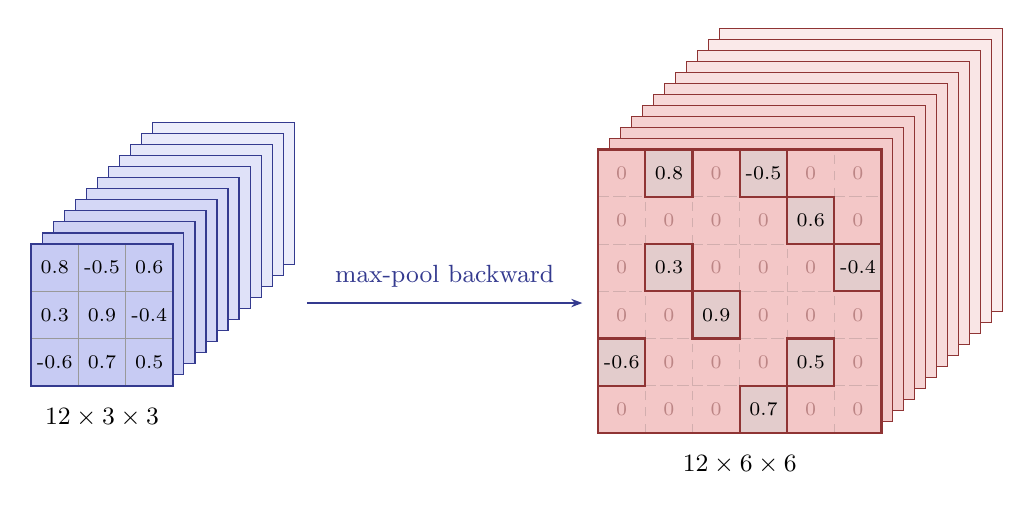
\begin{tikzpicture}[>={Stealth[length=4pt]}, line width=0.8pt, font=\large]

  % ================= 堆叠体：背面 11 层（★ 12 通道；左=紫系 3x3，右=红系 6x6） =================
  \foreach \k in {11,10,...,1}{
    \pgfmathtruncatemacro{\op}{100-6*\k}
    \fill[hidFill!\op, draw=hidLine, line width=0.4pt]
          ({0.14*\k},{0.6+0.14*\k}) rectangle ++(1.8,1.8);
    \fill[outFill!\op, draw=outLine, line width=0.4pt]
          ({7.2+0.14*\k},{0.14*\k}) rectangle ++(3.6,3.6);
  }

  % ================= 左正面：3x3 上游梯度（紫底） =================
  \fill[hidFill] (0,0.6) rectangle (1.8,2.4);
  \foreach \v [count=\n] in {0.8,-0.5,0.6, 0.3,0.9,-0.4, -0.6,0.7,0.5} {
    \pgfmathtruncatemacro{\r}{int((\n-1)/3)}
    \pgfmathtruncatemacro{\c}{mod(\n-1,3)}
    \draw[gray!80, line width=0.4pt] ({0.6*\c}, {0.6+0.6*(2-\r)}) rectangle ++(0.6,0.6);
    \node[font=\scriptsize] at ({0.6*\c+0.3}, {0.6+0.6*(2-\r)+0.3}) {\v};
  }
  \draw[hidLine] (0,0.6) rectangle (1.8,2.4);

  % ================= 右正面：6x6 稀疏梯度（红底） =================
  \fill[outFill] (7.2,0) rectangle (10.8,3.6);

  % ---- 第一遍：零格铺底（虚线 + 0） ----
  \foreach \v [count=\n] in \sparsevals {
    \pgfmathtruncatemacro{\r}{int((\n-1)/6)}
    \pgfmathtruncatemacro{\c}{mod(\n-1,6)}
    \pgfmathtruncatemacro{\nz}{abs(\v)>0.001?1:0}
    \ifnum\nz=0
      \draw[outLine!40, dashed, line width=0.3pt]
            ({7.2+0.6*\c}, {0.6*(5-\r)}) rectangle ++(0.6,0.6);
      \node[font=\scriptsize, text=outLine!60]
            at ({7.2+0.6*\c+0.3}, {0.6*(5-\r)+0.3}) {0};
    \fi
  }

  % ---- 第二遍：非零格盖顶（填充 + 实线框 + 数字） ----
  \foreach \v [count=\n] in \sparsevals {
    \pgfmathtruncatemacro{\r}{int((\n-1)/6)}
    \pgfmathtruncatemacro{\c}{mod(\n-1,6)}
    \pgfmathtruncatemacro{\nz}{abs(\v)>0.001?1:0}
    \ifnum\nz=1
      \fill[outLine!25] ({7.2+0.6*\c}, {0.6*(5-\r)}) rectangle ++(0.6,0.6);
      \draw[outLine, line width=0.8pt] ({7.2+0.6*\c}, {0.6*(5-\r)}) rectangle ++(0.6,0.6);
      \node[font=\scriptsize] at ({7.2+0.6*\c+0.3}, {0.6*(5-\r)+0.3}) {\v};
    \fi
  }

  \draw[outLine] (7.2,0) rectangle (10.8,3.6);

  % ================= 标题（★ 12 通道） =================
  \node[font=\small] at (0.9,0.2)  {$12\times3\times3$};
  \node[font=\small] at (9.0,-0.4)  {$12\times6\times6$};

  % ================= 箭头（紫指向红） =================
  \draw[hidLine, ->, line width=1pt] (3.5,1.65) -- (7.0,1.65)
    node[midway, above=2pt, font=\small] {max-pool backward};

\end{tikzpicture}
\end{document}